
%% bare_jrnl.tex
%% V1.3
%% 2007/01/11
%% by Michael Shell
%% see http://www.michaelshell.org/
%% for current contact information.
%%
%% This is a skeleton file demonstrating the use of IEEEtran.cls
%% (requires IEEEtran.cls version 1.7 or later) with an IEEE journal paper.
%%
%% Support sites:
%% http://www.michaelshell.org/tex/ieeetran/
%% http://www.ctan.org/tex-archive/macros/latex/contrib/IEEEtran/
%% and
%% http://www.ieee.org/



% *** Authors should verify (and, if needed, correct) their LaTeX system  ***
% *** with the testflow diagnostic prior to trusting their LaTeX platform ***
% *** with production work. IEEE's font choices can trigger bugs that do  ***
% *** not appear when using other class files.                            ***
% The testflow support page is at:
% http://www.michaelshell.org/tex/testflow/


%%*************************************************************************
%% Legal Notice:
%% This code is offered as-is without any warranty either expressed or
%% implied; without even the implied warranty of MERCHANTABILITY or
%% FITNESS FOR A PARTICULAR PURPOSE! 
%% User assumes all risk.
%% In no event shall IEEE or any contributor to this code be liable for
%% any damages or losses, including, but not limited to, incidental,
%% consequential, or any other damages, resulting from the use or misuse
%% of any information contained here.
%%
%% All comments are the opinions of their respective authors and are not
%% necessarily endorsed by the IEEE.
%%
%% This work is distributed under the LaTeX Project Public License (LPPL)
%% ( http://www.latex-project.org/ ) version 1.3, and may be freely used,
%% distributed and modified. A copy of the LPPL, version 1.3, is included
%% in the base LaTeX documentation of all distributions of LaTeX released
%% 2003/12/01 or later.
%% Retain all contribution notices and credits.
%% ** Modified files should be clearly indicated as such, including  **
%% ** renaming them and changing author support contact information. **
%%
%% File list of work: IEEEtran.cls, IEEEtran_HOWTO.pdf, bare_adv.tex,
%%                    bare_conf.tex, bare_jrnl.tex, bare_jrnl_compsoc.tex
%%*************************************************************************

% Note that the a4paper option is mainly intended so that authors in
% countries using A4 can easily print to A4 and see how their papers will
% look in print - the typesetting of the document will not typically be
% affected with changes in paper size (but the bottom and side margins will).
% Use the testflow package mentioned above to verify correct handling of
% both paper sizes by the user's LaTeX system.
%
% Also note that the "draftcls" or "draftclsnofoot", not "draft", option
% should be used if it is desired that the figures are to be displayed in
% draft mode.
%
\documentclass[journal]{IEEEtran}
%
% If IEEEtran.cls has not been installed into the LaTeX system files,
% manually specify the path to it like:
% \documentclass[journal]{../sty/IEEEtran}





% Some very useful LaTeX packages include:
% (uncomment the ones you want to load)


% *** MISC UTILITY PACKAGES ***
%
%\usepackage{ifpdf}
% Heiko Oberdiek's ifpdf.sty is very useful if you need conditional
% compilation based on whether the output is pdf or dvi.
% usage:
% \ifpdf
%   % pdf code
% \else
%   % dvi code
% \fi
% The latest version of ifpdf.sty can be obtained from:
% http://www.ctan.org/tex-archive/macros/latex/contrib/oberdiek/
% Also, note that IEEEtran.cls V1.7 and later provides a builtin
% \ifCLASSINFOpdf conditional that works the same way.
% When switching from latex to pdflatex and vice-versa, the compiler may
% have to be run twice to clear warning/error messages.






% *** CITATION PACKAGES ***
%
%\usepackage{cite}
% cite.sty was written by Donald Arseneau
% V1.6 and later of IEEEtran pre-defines the format of the cite.sty package
% \cite{} output to follow that of IEEE. Loading the cite package will
% result in citation numbers being automatically sorted and properly
% "compressed/ranged". e.g., [1], [9], [2], [7], [5], [6] without using
% cite.sty will become [1], [2], [5]--[7], [9] using cite.sty. cite.sty's
% \cite will automatically add leading space, if needed. Use cite.sty's
% noadjust option (cite.sty V3.8 and later) if you want to turn this off.
% cite.sty is already installed on most LaTeX systems. Be sure and use
% version 4.0 (2003-05-27) and later if using hyperref.sty. cite.sty does
% not currently provide for hyperlinked citations.
% The latest version can be obtained at:
% http://www.ctan.org/tex-archive/macros/latex/contrib/cite/
% The documentation is contained in the cite.sty file itself.






% *** GRAPHICS RELATED PACKAGES ***
%
\ifCLASSINFOpdf
  \usepackage[pdftex]{graphicx}
  % declare the path(s) where your graphic files are
  % graphicspath{{../pdf/}{../jpeg/}}
  % and their extensions so you won't have to specify these with
  % every instance of \includegraphics
  \DeclareGraphicsExtensions{.pdf,.jpeg,.png}
\else
  % or other class option (dvipsone, dvipdf, if not using dvips). graphicx
  % will default to the driver specified in the system graphics.cfg if no
  % driver is specified.
  % \usepackage[dvips]{graphicx}
  % declare the path(s) where your graphic files are
  % \graphicspath{{../eps/}}
  % and their extensions so you won't have to specify these with
  % every instance of \includegraphics
  % \DeclareGraphicsExtensions{.eps}
\fi
% graphicx was written by David Carlisle and Sebastian Rahtz. It is
% required if you want graphics, photos, etc. graphicx.sty is already
% installed on most LaTeX systems. The latest version and documentation can
% be obtained at: 
% http://www.ctan.org/tex-archive/macros/latex/required/graphics/
% Another good source of documentation is "Using Imported Graphics in
% LaTeX2e" by Keith Reckdahl which can be found as epslatex.ps or
% epslatex.pdf at: http://www.ctan.org/tex-archive/info/
%
% latex, and pdflatex in dvi mode, support graphics in encapsulated
% postscript (.eps) format. pdflatex in pdf mode supports graphics
% in .pdf, .jpeg, .png and .mps (metapost) formats. Users should ensure
% that all non-photo figures use a vector format (.eps, .pdf, .mps) and
% not a bitmapped formats (.jpeg, .png). IEEE frowns on bitmapped formats
% which can result in "jaggedy"/blurry rendering of lines and letters as
% well as large increases in file sizes.
%
% You can find documentation about the pdfTeX application at:
% http://www.tug.org/applications/pdftex





% *** MATH PACKAGES ***
%
%\usepackage[cmex10]{amsmath}
% A popular package from the American Mathematical Society that provides
% many useful and powerful commands for dealing with mathematics. If using
% it, be sure to load this package with the cmex10 option to ensure that
% only type 1 fonts will utilized at all point sizes. Without this option,
% it is possible that some math symbols, particularly those within
% footnotes, will be rendered in bitmap form which will result in a
% document that can not be IEEE Xplore compliant!
%
% Also, note that the amsmath package sets \interdisplaylinepenalty to 10000
% thus preventing page breaks from occurring within multiline equations. Use:
%\interdisplaylinepenalty=2500
% after loading amsmath to restore such page breaks as IEEEtran.cls normally
% does. amsmath.sty is already installed on most LaTeX systems. The latest
% version and documentation can be obtained at:
% http://www.ctan.org/tex-archive/macros/latex/required/amslatex/math/





% *** SPECIALIZED LIST PACKAGES ***
%
%\usepackage{algorithmic}
% algorithmic.sty was written by Peter Williams and Rogerio Brito.
% This package provides an algorithmic environment fo describing algorithms.
% You can use the algorithmic environment in-text or within a figure
% environment to provide for a floating algorithm. Do NOT use the algorithm
% floating environment provided by algorithm.sty (by the same authors) or
% algorithm2e.sty (by Christophe Fiorio) as IEEE does not use dedicated
% algorithm float types and packages that provide these will not provide
% correct IEEE style captions. The latest version and documentation of
% algorithmic.sty can be obtained at:
% http://www.ctan.org/tex-archive/macros/latex/contrib/algorithms/
% There is also a support site at:
% http://algorithms.berlios.de/index.html
% Also of interest may be the (relatively newer and more customizable)
% algorithmicx.sty package by Szasz Janos:
% http://www.ctan.org/tex-archive/macros/latex/contrib/algorithmicx/




% *** ALIGNMENT PACKAGES ***
%
%\usepackage{array}
% Frank Mittelbach's and David Carlisle's array.sty patches and improves
% the standard LaTeX2e array and tabular environments to provide better
% appearance and additional user controls. As the default LaTeX2e table
% generation code is lacking to the point of almost being broken with
% respect to the quality of the end results, all users are strongly
% advised to use an enhanced (at the very least that provided by array.sty)
% set of table tools. array.sty is already installed on most systems. The
% latest version and documentation can be obtained at:
% http://www.ctan.org/tex-archive/macros/latex/required/tools/


%\usepackage{mdwmath}
%\usepackage{mdwtab}
% Also highly recommended is Mark Wooding's extremely powerful MDW tools,
% especially mdwmath.sty and mdwtab.sty which are used to format equations
% and tables, respectively. The MDWtools set is already installed on most
% LaTeX systems. The lastest version and documentation is available at:
% http://www.ctan.org/tex-archive/macros/latex/contrib/mdwtools/


% IEEEtran contains the IEEEeqnarray family of commands that can be used to
% generate multiline equations as well as matrices, tables, etc., of high
% quality.


%\usepackage{eqparbox}
% Also of notable interest is Scott Pakin's eqparbox package for creating
% (automatically sized) equal width boxes - aka "natural width parboxes".
% Available at:
% http://www.ctan.org/tex-archive/macros/latex/contrib/eqparbox/





% *** SUBFIGURE PACKAGES ***
%\usepackage[tight,footnotesize]{subfigure}
% subfigure.sty was written by Steven Douglas Cochran. This package makes it
% easy to put subfigures in your figures. e.g., "Figure 1a and 1b". For IEEE
% work, it is a good idea to load it with the tight package option to reduce
% the amount of white space around the subfigures. subfigure.sty is already
% installed on most LaTeX systems. The latest version and documentation can
% be obtained at:
% http://www.ctan.org/tex-archive/obsolete/macros/latex/contrib/subfigure/
% subfigure.sty has been superceeded by subfig.sty.



%\usepackage[caption=false]{caption}
%\usepackage[font=footnotesize]{subfig}
% subfig.sty, also written by Steven Douglas Cochran, is the modern
% replacement for subfigure.sty. However, subfig.sty requires and
% automatically loads Axel Sommerfeldt's caption.sty which will override
% IEEEtran.cls handling of captions and this will result in nonIEEE style
% figure/table captions. To prevent this problem, be sure and preload
% caption.sty with its "caption=false" package option. This is will preserve
% IEEEtran.cls handing of captions. Version 1.3 (2005/06/28) and later 
% (recommended due to many improvements over 1.2) of subfig.sty supports
% the caption=false option directly:
%\usepackage[caption=false,font=footnotesize]{subfig}
%
% The latest version and documentation can be obtained at:
% http://www.ctan.org/tex-archive/macros/latex/contrib/subfig/
% The latest version and documentation of caption.sty can be obtained at:
% http://www.ctan.org/tex-archive/macros/latex/contrib/caption/




% *** FLOAT PACKAGES ***
%
%\usepackage{fixltx2e}
% fixltx2e, the successor to the earlier fix2col.sty, was written by
% Frank Mittelbach and David Carlisle. This package corrects a few problems
% in the LaTeX2e kernel, the most notable of which is that in current
% LaTeX2e releases, the ordering of single and double column floats is not
% guaranteed to be preserved. Thus, an unpatched LaTeX2e can allow a
% single column figure to be placed prior to an earlier double column
% figure. The latest version and documentation can be found at:
% http://www.ctan.org/tex-archive/macros/latex/base/



%\usepackage{stfloats}
% stfloats.sty was written by Sigitas Tolusis. This package gives LaTeX2e
% the ability to do double column floats at the bottom of the page as well
% as the top. (e.g., "\begin{figure*}[!b]" is not normally possible in
% LaTeX2e). It also provides a command:
%\fnbelowfloat
% to enable the placement of footnotes below bottom floats (the standard
% LaTeX2e kernel puts them above bottom floats). This is an invasive package
% which rewrites many portions of the LaTeX2e float routines. It may not work
% with other packages that modify the LaTeX2e float routines. The latest
% version and documentation can be obtained at:
% http://www.ctan.org/tex-archive/macros/latex/contrib/sttools/
% Documentation is contained in the stfloats.sty comments as well as in the
% presfull.pdf file. Do not use the stfloats baselinefloat ability as IEEE
% does not allow \baselineskip to stretch. Authors submitting work to the
% IEEE should note that IEEE rarely uses double column equations and
% that authors should try to avoid such use. Do not be tempted to use the
% cuted.sty or midfloat.sty packages (also by Sigitas Tolusis) as IEEE does
% not format its papers in such ways.


%\ifCLASSOPTIONcaptionsoff
%  \usepackage[nomarkers]{endfloat}
% \let\MYoriglatexcaption\caption
% \renewcommand{\caption}[2][\relax]{\MYoriglatexcaption[#2]{#2}}
%\fi
% endfloat.sty was written by James Darrell McCauley and Jeff Goldberg.
% This package may be useful when used in conjunction with IEEEtran.cls'
% captionsoff option. Some IEEE journals/societies require that submissions
% have lists of figures/tables at the end of the paper and that
% figures/tables without any captions are placed on a page by themselves at
% the end of the document. If needed, the draftcls IEEEtran class option or
% \CLASSINPUTbaselinestretch interface can be used to increase the line
% spacing as well. Be sure and use the nomarkers option of endfloat to
% prevent endfloat from "marking" where the figures would have been placed
% in the text. The two hack lines of code above are a slight modification of
% that suggested by in the endfloat docs (section 8.3.1) to ensure that
% the full captions always appear in the list of figures/tables - even if
% the user used the short optional argument of \caption[]{}.
% IEEE papers do not typically make use of \caption[]'s optional argument,
% so this should not be an issue. A similar trick can be used to disable
% captions of packages such as subfig.sty that lack options to turn off
% the subcaptions:
% For subfig.sty:
% \let\MYorigsubfloat\subfloat
% \renewcommand{\subfloat}[2][\relax]{\MYorigsubfloat[]{#2}}
% For subfigure.sty:
% \let\MYorigsubfigure\subfigure
% \renewcommand{\subfigure}[2][\relax]{\MYorigsubfigure[]{#2}}
% However, the above trick will not work if both optional arguments of
% the \subfloat/subfig command are used. Furthermore, there needs to be a
% description of each subfigure *somewhere* and endfloat does not add
% subfigure captions to its list of figures. Thus, the best approach is to
% avoid the use of subfigure captions (many IEEE journals avoid them anyway)
% and instead reference/explain all the subfigures within the main caption.
% The latest version of endfloat.sty and its documentation can obtained at:
% http://www.ctan.org/tex-archive/macros/latex/contrib/endfloat/
%
% The IEEEtran \ifCLASSOPTIONcaptionsoff conditional can also be used
% later in the document, say, to conditionally put the References on a 
% page by themselves.





% *** PDF, URL AND HYPERLINK PACKAGES ***
%
\usepackage{url}
\usepackage{hyperref}
% url.sty was written by Donald Arseneau. It provides better support for
% handling and breaking URLs. url.sty is already installed on most LaTeX
% systems. The latest version can be obtained at:
% http://www.ctan.org/tex-archive/macros/latex/contrib/misc/
% Read the url.sty source comments for usage information. Basically,
% \url{my_url_here}.


% Listings
\usepackage{listings}


% *** Do not adjust lengths that control margins, column widths, etc. ***
% *** Do not use packages that alter fonts (such as pslatex).         ***
% There should be no need to do such things with IEEEtran.cls V1.6 and later.
% (Unless specifically asked to do so by the journal or conference you plan
% to submit to, of course. )


% correct bad hyphenation here
\hyphenation{op-tical net-works semi-conduc-tor}


\begin{document}
\lstset{language=HTML}  

%
% paper title
% can use linebreaks \\ within to get better formatting as desired
\title{Viability of HTML5 video as a replacement for plug-in based approaches of delivering video content to user agents}
%
%
% author names and IEEE memberships
% note positions of commas and nonbreaking spaces ( ~ ) LaTeX will not break
% a structure at a ~ so this keeps an author's name from being broken across
% two lines.
% use \thanks{} to gain access to the first footnote area
% a separate \thanks must be used for each paragraph as LaTeX2e's \thanks
% was not built to handle multiple paragraphs
%

%\author{Michael~Shell,~\IEEEmembership{Member,~IEEE,}
%        John~Doe,~\IEEEmembership{Fellow,~OSA,}
%        and~Jane~Doe,~\IEEEmembership{Life~Fellow,~IEEE}% <-this % stops a space
\author{David~Hulme%
\thanks{K. Martinez is with the Department
of Electronics and Computer Science, University of Southampton, UK e-mail: (see http://users.ecs.soton.ac.uk/km).}}% <-this % stops a space
%\thanks{J. Doe and J. Doe are with Anonymous University.}% <-this % stops a space
%\thanks{Manuscript received April 19, 2005; revised January 11, 2007.}}

% note the % following the last \IEEEmembership and also \thanks - 
% these prevent an unwanted space from occurring between the last author name
% and the end of the author line. i.e., if you had this:
% 
% \author{....lastname \thanks{...} \thanks{...} }
%                     ^------------^------------^----Do not want these spaces!
%
% a space would be appended to the last name and could cause every name on that
% line to be shifted left slightly. This is one of those "LaTeX things". For
% instance, "\textbf{A} \textbf{B}" will typeset as "A B" not "AB". To get
% "AB" then you have to do: "\textbf{A}\textbf{B}"
% \thanks is no different in this regard, so shield the last } of each \thanks
% that ends a line with a % and do not let a space in before the next \thanks.
% Spaces after \IEEEmembership other than the last one are OK (and needed) as
% you are supposed to have spaces between the names. For what it is worth,
% this is a minor point as most people would not even notice if the said evil
% space somehow managed to creep in.



% The paper headers
%\markboth{Journal of \LaTeX\ Class Files,~Vol.~6, No.~1, January~2007}%
%{Shell \MakeLowercase{\textit{et al.}}: Bare Demo of IEEEtran.cls for Journals}
% The only time the second header will appear is for the odd numbered pages
% after the title page when using the twoside option.
% 
% *** Note that you probably will NOT want to include the author's ***
% *** name in the headers of peer review papers.                   ***
% You can use \ifCLASSOPTIONpeerreview for conditional compilation here if
% you desire.




% If you want to put a publisher's ID mark on the page you can do it like
% this:
%\IEEEpubid{0000--0000/00\$00.00~\copyright~2007 IEEE}
% Remember, if you use this you must call \IEEEpubidadjcol in the second
% column for its text to clear the IEEEpubid mark.



% use for special paper notices
%\IEEEspecialpapernotice{(Invited Paper)}




% make the title area
\maketitle


\begin{abstract}
%\boldmath
HTML5 defines a method for videos to be embedded directly into a web page. The ability to directly embed videos into web pages removes the web browser's dependence on third party software and opens new possibilities for the integration of video multimedia with other web content.

However, for any new web technology to gain acceptance it must be comparable to the current technology in use. In this paper, an examination on the viability of HTML5 video as a replacement for the current plug-in based technologies in use is conducted as well as research into what new opportunities it can provide.
\end{abstract}

\IEEEpeerreviewmaketitle

\section{Introduction}
\IEEEPARstart{I}{nternet} video traffic is growing. Cisco predict that by 2017, consumer Internet video traffic will account for 69\% of all consumer internet traffic \cite{website:ciscoForecastAndMethodology}. In addition, nearly half of all internet traffic will originate from a non-PC device \cite{website:ciscoForecastAndMethodology}. It is therefore important to ensure that technologies are in place to deliver this content to users and provide a high quality viewing experience across a wide range of devices and platforms.

A typical way users access video multimedia is through an embedded video on a web page. Typically this has been achieved through the use of third party plug-ins such as Adobe Flash\footnote{Adobe Flash Player: \url{http://www.adobe.com/uk/software/flash/about/}}, henceforth referred to as Flash, or Microsoft Silverlight\footnote{Microsoft Silverlight: \url{http://www.microsoft.com/silverlight/}}, now referred to as Silverlight. Flash was well on the way to becoming the de facto standard for embedding video into web pages \cite{article:HTML5LeadsAWebRevolution}. However, in 2010 Apple announced that they would not allow Flash on their mobile devices, citing the closed nature of Flash, reliability, security and performance as concerns \cite{website:appleFlash}. Watanabe et al. also raised concerns regarding the security of Flash \cite{inproceedings:flashSecurity}. An industry agreed standard addressing these concerns is required.

HTML5, an emerging specification from the W3C, includes a \texttt{video} element definition. This element enables videos to be embedded directly into a web page\cite{standard:html5}. Natively embedding videos into web pages removes the web browser's dependence on a third party plug-in, increasing openness. %more benefits?
In addition it opens new possibilities for the integration of video multimedia with other web content.

However, any replacement for embedding video content must be suitable and comparable to the current technology in use. This paper will research key areas relating to the delivery of video content to user agents and the subsequent user interaction with the video to examine whether HTML5 video is a viable replacement for the current plug-in based technologies in use.

\section{Content Delivery}
% something to go here
\subsection{Embedding Method}
HTML5 specifies the \textless object\textgreater tag which allows for external resources to be embedded in a web page that are processed by a plug-in \cite{standard:html5}. As Daoust et al. noted, ``relying on third-party plug-ins to render the video works fine in a variety of use cases'' \cite{article:towardsVideoOnTheWebWithHTML5}. However, they also stated that because the video is rendered in a black box, from the browser's perspective, CSS and SVG cannot be used to style the video or apply visual effects \cite{article:towardsVideoOnTheWebWithHTML5}. The \textless video\textgreater tag directly integrates the video into the browser, alleviating these problems.

The native embedding of a video in the browser allows for improved interaction between the video and other elements in the page. Oehme et al. used this native integration to add dynamic overlays to a video containing related data from various internet sources \cite{inproceedings:theChroomaApproach}. Other applications are possible with HTML5 \textless canvas\textgreater tag, that ``provides scripts with a resolution-dependent bitmap canvas'' to which visual images can be rendered to \cite{standard:html5}. Fulton, S. and Fulton, J. describe how a canvas video puzzle application can be created by using created using this interaction \cite{book:html5canvas}. Quax et al. used a hidden video element to receive a video stream from the server. They then manipulated the video before displaying it on a canvas element \cite{inproceedings:aPracticalAndScableMethodForStreaming}.

\subsection{Supported Formats}
An important distinction to first make is the difference between a video container and a codec. A codec is the format in which the audio or video is encoded. Some example video codecs include H.264, Theora, VP6 and VP8. A container describes the structure of the file and what codecs are in use \cite{website:videoFormatsGuide}. Some example containers include MP4, WebM, Ogg, AVI and FLV.

Flash only plays videos contained within the FLV (Flash Video) container or the ShockWave Flash format used in earlier releases \cite{article:flashPlayer}. Flash supports the VP6 and Spark codecs \cite{article:flashPlayer} and since version 9 supports H.264 \cite{website:flashSupportedFormats}. Silverlight supports the ASF, MP4 and 3GP containers and supports a variety of codecs including H.264 and WMV \cite{website:silverlightSupportedFormats}.

HTML5 does not specify support for any specific codec or container format \cite{article:towardsVideoOnTheWebWithHTML5}. The three main codecs and containers currently supported are H.264 in an MP4 container, Theora in an Ogg container and VP8 in a WebM container \cite{article:towardsVideoOnTheWebWithHTML5}.

Table \ref{tab:supportedCodecsAndContainers} shows the support for these three formats across different browsers. Data is sourced from  \cite{inproceedings:applicationOfHTML5Multimedia} and  \cite{article:towardsVideoOnTheWebWithHTML5}. It is important to note that Table \ref{tab:supportedCodecsAndContainers} only considers that a format is supported if it is supported natively by the browser, for example Firefox relies on a Flash fall back to play H.264 content \cite{website:firefoxVideoMobileAndTheOpenWeb}.

\begin{table}
	\label{tab:supportedCodecsAndContainers}
	\caption{Supported Codecs and Containers by Browser}
    \begin{tabular}{|l|l|l|l|}
    \hline
    \textbf{Browser}    & \textbf{H.264 in MP4} & \textbf{Theora in Ogg} & \textbf{VP8 in WebM} \\ \hline
    IE8        & No           & No            & No          \\ \hline
    IE9+       & Yes          & No            & No          \\ \hline
    Chrome 18+ & Yes          & Yes           & Yes         \\ \hline
    Firefox 6+ & No           & Yes           & Yes         \\ \hline
    Opera 12+  & No           & Yes           & Yes         \\ \hline
    Safari 5+  & Yes          & No            & No          \\ \hline
    \end{tabular}
\end{table}

Table \ref{tab:supportedCodecsAndContainers} illustrates how there is inconsistent support for different formats across browsers. The problems around these codecs are caused by patents and licensing fees. H.264 is not royalty free and although VP8 and Theora have been released with royalty-free licences, Intellectual Property Rights holders may appear in the future \cite{article:towardsVideoOnTheWebWithHTML5} \cite{website:theoraBenefits}. To ensure that a video is playable across multiple browsers, developers can specify multiple \textless source\textgreater~tags within the \textless video\textgreater~tag that specify different formats of the video that are available. The browser is then able to choose to play the format it most prefers. An example of this is shown in Figure \ref{lst:HTML5VideoExample}. If the browser does not support HTML5 video then the \textless object\textgreater~tag, which embeds a flash video, will be rendered instead.

\begin{figure}
\label{lst:HTML5VideoExample}
\caption{HTML5 Video Example}
\begin{lstlisting}[frame=single]
<video>
 <source src="video.mp4" type="video/mp4">
 <source src="video.ogg" type="video/ogg">
 <source src="video.webm" type="video/webm">
 <object>
  <param name="movie" value="movie.flv">
 </object>
</video>
\end{lstlisting}
\end{figure}

\subsection{Delivery Methods}
% I think these links should probs be footnotes
There are two distinct approaches for delivering video content to clients. The first is traditional streaming through protocols such as Real Time Streaming Protocol (RTSP) \cite{misc:rfcRSTP} with Real-time Transport Protocol (RTP) \cite{misc:rfcRTP} or Adobe's Real Time Message Protocol (RTMP)\cite{website:RTMP} \cite{article:areWeInTheMiddleOfAVideoStreamingRevolution}. These are push-based streaming protocols where the ``server streams packets to the client until the client interrupts or stops the session'' \cite{article:watchingVideoOverTheWeb} with the client not store storing the file on their machine. A media server is required to manage the streams, an approach traditionally used by Flash \cite{article:flashPlayer}.

The second are pulled-based approaches usually over the HTTP protocol. The simplest of these is progressive download where the client begins downloading the video and begins play when it has reached a minimum threshold \cite{article:watchingVideoOverTheWeb}. However with this approach the client is unable to jump to a point in the video that has not downloaded and there is no guarantee that the delivery rate will remain constant \cite{article:towardsVideoOnTheWebWithHTML5}.  Therefore more intelligent, adaptive streaming technologies have been developed such as Apple's HTTP Live Streaming (HLS) \cite{misc:HTTPLiveStreaming}, Adobe's Dynamic HTTP Streaming \cite{website:HTTPDynamicStreaming} or Microsoft's Smooth Streaming \cite{website:smoothStreaming} \cite{inproceedings:aSeamlessIntegrationOfAdaptiveHTTPStreaming}. Content is delivered through a Content Delivery Network (CDN) which can improve caching, efficiency and reduce licensing costs \cite{article:towardsVideoOnTheWebWithHTML5}\cite{inproceedings:HTTPAsTheNarrowWaist}.

HTML5 video does not declare if implementations should support streaming through protocols other than HTTP - currently most browsers do not. %citation?
Consequently video streaming in HTML5 must be done over HTTP.

% there was lots other stuff to talk about here... will come back to it.

\subsection{Content Protection}

\section{Performance}
Globally, mobile data traffic will increase 13-fold between 2012 and 2017 \cite{website:ciscoForecastAndMethodology}. This will lead to an increasing amount of internet video being consumed on mobile devices. Such devices will be less powerful than the typical desktop computer and will have an emphasis on optimising their battery life. It is important that watching an HTML5 video is not a large drain on resources. % could probably say this better.

Ilias et al. conducted a study to analyse the video streaming performance between Flash video and HTML5 video \cite{inproceedings:aStudyOfVideoPerformanceAnalysis}. They looked at two video performance metrics, frame rate and CPU usage, whilst streaming a video over wired and wireless networks across a variety of browsers. Their study showed that the implementation of HTML5 video in each browser had a big effect on the performance. This can be seen in Figure \ref{fig:cpuPerformanceGraph}. Overall the average CPU for Flash was 77\% and 87\% for HTML5 video. This shows that on average, HTML5 video requires 13\% more CPU power than Flash. In addition, in IE9 HTML5 video used 95\% of the CPU. This certainly has the potential to cause playback problems on mobile devices and cause frustration to users. However, the HTML5 video Chrome result suggests that the CPU usage is heavily influenced by the HTML5 video implementation. Thus over time, the situation should improve.

% could look at native decoder chips, hardware vs software decoding
% maybe there also some additional studies on latency etc. 

\begin{figure}[!t]
\centering
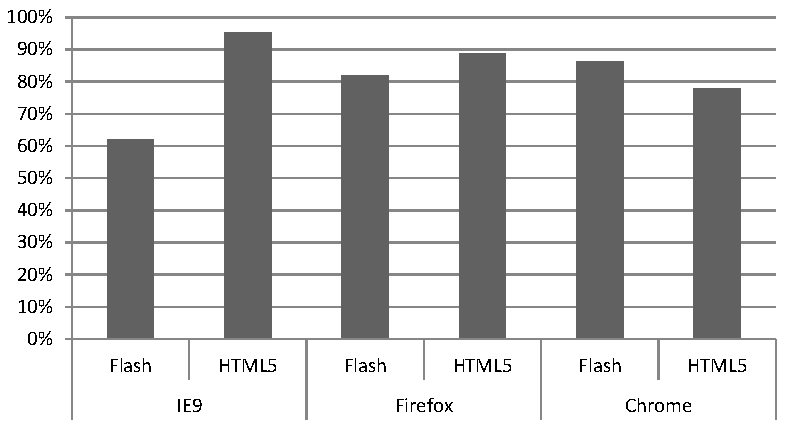
\includegraphics[width=3.5in]{cpu-performance-graph}
\caption{CPU usage across different browsers. Data produced by averaging results from Ilias et al. \cite{inproceedings:aStudyOfVideoPerformanceAnalysis} across two different CPU monitoring tools and both wired and wireless networks.}
\label{fig:cpuPerformanceGraph}
\end{figure} 

\section{Accessibility}
Accessibility on the web is governed by the W3C 2008 recommendation, Web Content Accessibility Guidelines (WCAG)\footnote{Web Content Accessibility Guidelines (WCAG) 2.0: \url{http://www.w3.org/TR/WCAG20/}}. More recently, The User Agent Accessibility Guidelines (UAAG), a standard to provide additional advice on the application user interface is in development \cite{website:implementingUAAG}.

% did they actually propose it?
Moreno et al. propose three areas that must be considered to deliver accessible multimedia content: accessible video, accessible web page and accessible user interaction \cite{article:disablityStandardsForMultimediaOnTheWeb}.

\subsection{Accessible Video}
WCAG 2.0 Guideline 1.2 requires that developers provide alternatives for time-based media such as alternative text, captions, audio description and sign language as shown in Table \ref{tab:wcag2Guidelines} \cite{standard:wcag2}.

\begin{table}
  \caption{WCAG 2.0 Guidelines\cite{standard:wcag2}}
  \label{tab:wcag2Guidelines}
    \begin{tabular}{|l|l|l|}
    \hline
    \textbf{Guideline}          & \textbf{Type} & \textbf{Conformance level} \\ \hline
    1.1.1 Non-text Content                 & All         & A                 \\ \hline
    1.2.1 Alternative for time-based media & Prerecorded & A                 \\ \hline
    1.2.2 Captions                         & Prerecorded & A                 \\ \hline
    1.2.4 Captions                         & Live        & AA                \\ \hline
    1.2.5 Audio Description                & Prerecorded & AA                \\ \hline
    1.2.6 Sign Language                    & Prerecorded & AAA               \\ \hline
    \end{tabular}
\end{table}

The W3C provides documents detailing how these guidelines can be met for different technologies such as Flash and Silverlight \footnote{Flash Techniques for WCAG 2.0: \url{http://www.w3.org/TR/WCAG20-TECHS/flash.html}} \footnote{Silverlight Techniques for WCAG 2.0: \url{http://www.w3.org/TR/WCAG20-TECHS/silverlight.html}}. For example the Flash document explains how developers can add subtitles to their Flash videos using an XML file to meet WCAG 2.0 Guideline 1.2.2 \cite{website:flashTechniquesForWCAG}.

Pfeiffer and Parker describe existing implementations for supporting subtitles for HTML5 video \cite{inproceedings:accessibilityForTheHTML5VideoElement}. They describe the work of Jan Gerber who uses JavaScript to load subtitles from a text file and display them on screen in time with an HTML5 video\footnote{Jan Gerber, jquery.srt.js: \url{http://v2v.cc/~j/jquery.srt/}} \cite{inproceedings:accessibilityForTheHTML5VideoElement}. HTML5 specifies a \textless track\textgreater tag that can be used to specify timed text tracks for media elements, see Figure \ref{lst:trackExample} \cite{standard:html5}. Currently implementations vary by browser and cross-browser native support the track element is some way off. %citation?

% could mention using webvtt format?

\begin{figure}
\label{lst:trackExample}
\caption{HTML5 Track Example}
\begin{lstlisting}[frame=single]
<video>
  <source src="video.webm">
  <track src="subtitles.vtt"
    label="English subtitles"
     kind="subtitles" srclang="en">
  </track>
</video>
\end{lstlisting}
\end{figure}

% could also talk about embedding in file....
%Instead of accessibility data can be stored within container formats such as Ogg %\cite{inproceedings:accessibilityForTheHTML5VideoElement}. 
% http://git.xiph.org/?p=ffmpeg2theora.git;a=blob_plain;f=subtitles.txt;hb=HEAD

\subsection{Accessible Web Page}
% web page 
% how embedded in web page
% not sure what to say here, may remove it

\subsection{Accessible User Interaction}
% user interaction
% interaction with user - clicking buttons etc
WCAG 2.0 Guideline 2.2.2 states that for any moving content, there must exist some mechanism to pause the content. Mostly all video embedding solutions provide this. Guideline 2.1.1 states that all content must be operable through the keyboard \cite{standard:wcag2}. One of the key problems with plug-in based approaches such as Flash or Silverlight is that any video playback controls are generally inaccessible to screen readers who read web pages based on HTML tags \cite{inproceedings:transformingFlashToXML} \cite{incollection:accessibilityEvaluationForMultimediaContent}. Plug-in content is delivered in a binary format and determining the structure of the content at runtime is near impossible \cite{inproceedings:transformingFlashToXML}.

Adobe has provided a document, ``Best Practices for Accessible Flash Design'' which describes how Flash content can be understood by screen readers through Microsoft Active Accessibility\footnote{Microsoft Active Accessibility: \url{http://msdn.microsoft.com/en-us/library/windows/desktop/dd373592(v=vs.85).aspx
}} (MSAA) \cite{whitePaper:bestPracticesForAccessibleFlashDesign}. If an author of Flash content adds the required accessibility information into the content, Flash can expose their content to screen readers \cite{inproceedings:automaticAccesibilityTranscodingForFlashContent}.

% maybe I try and duplicate their findings?
However there are some limitations with this system. Flash exposes information for buttons even if the button has no active behaviour. Sato et al. found that the MSAA information for the Flash YouTube player states that there are 13 buttons in the player, where in fact there are only 5 shown to users. Some of the 13 buttons had no functional content and others had no keyboard access and so were inaccessible to blind users \cite{inproceedings:automaticAccesibilityTranscodingForFlashContent}.

% could talk about the survey in 'accessibility evaluation for multiemedia content'. but this was a while ago, so may not be relevant anymore?

In HTML5, default video controls can be included using the `controls' attribute on the \textless video\textgreater tag. However since these controls are not all contrable via the keyboard %citation
they do not meet accessibility guidelines. Moreno et al. developed an accessible HTML5 video player by adding HTML buttons to control the video player that can be controlled by a screen reader\cite{incollection:html5SupportForAnAccessibleWeb}.

In conclusion, accessible environments are most easily achieved through the use of HTML pages created according to Web content accessibility guidelines \cite{incollection:accessibilityEvaluationForMultimediaContent}.

\section{Conclusion}
The conclusion goes here.



% An example of a floating figure using the graphicx package.
% Note that \label must occur AFTER (or within) \caption.
% For figures, \caption should occur after the \includegraphics.
% Note that IEEEtran v1.7 and later has special internal code that
% is designed to preserve the operation of \label within \caption
% even when the captionsoff option is in effect. However, because
% of issues like this, it may be the safest practice to put all your
% \label just after \caption rather than within \caption{}.
%
% Reminder: the "draftcls" or "draftclsnofoot", not "draft", class
% option should be used if it is desired that the figures are to be
% displayed while in draft mode.
%
%\begin{figure}[!t]
%\centering
%\includegraphics[width=2.5in]{myfigure}
% where an .eps filename suffix will be assumed under latex, 
% and a .pdf suffix will be assumed for pdflatex; or what has been declared
% via \DeclareGraphicsExtensions.
%\caption{Simulation Results}
%\label{fig_sim}
%\end{figure}

% Note that IEEE typically puts floats only at the top, even when this
% results in a large percentage of a column being occupied by floats.


% An example of a double column floating figure using two subfigures.
% (The subfig.sty package must be loaded for this to work.)
% The subfigure \label commands are set within each subfloat command, the
% \label for the overall figure must come after \caption.
% \hfil must be used as a separator to get equal spacing.
% The subfigure.sty package works much the same way, except \subfigure is
% used instead of \subfloat.
%
%\begin{figure*}[!t]
%\centerline{\subfloat[Case I]\includegraphics[width=2.5in]{subfigcase1}%
%\label{fig_first_case}}
%\hfil
%\subfloat[Case II]{\includegraphics[width=2.5in]{subfigcase2}%
%\label{fig_second_case}}}
%\caption{Simulation results}
%\label{fig_sim}
%\end{figure*}
%
% Note that often IEEE papers with subfigures do not employ subfigure
% captions (using the optional argument to \subfloat), but instead will
% reference/describe all of them (a), (b), etc., within the main caption.


% An example of a floating table. Note that, for IEEE style tables, the 
% \caption command should come BEFORE the table. Table text will default to
% \footnotesize as IEEE normally uses this smaller font for tables.
% The \label must come after \caption as always.
%
%\begin{table}[!t]
%% increase table row spacing, adjust to taste
%\renewcommand{\arraystretch}{1.3}
% if using array.sty, it might be a good idea to tweak the value of
% \extrarowheight as needed to properly center the text within the cells
%\caption{An Example of a Table}
%\label{table_example}
%\centering
%% Some packages, such as MDW tools, offer better commands for making tables
%% than the plain LaTeX2e tabular which is used here.
%\begin{tabular}{|c||c|}
%\hline
%One & Two\\
%\hline
%Three & Four\\
%\hline
%\end{tabular}
%\end{table}


% Note that IEEE does not put floats in the very first column - or typically
% anywhere on the first page for that matter. Also, in-text middle ("here")
% positioning is not used. Most IEEE journals use top floats exclusively.
% Note that, LaTeX2e, unlike IEEE journals, places footnotes above bottom
% floats. This can be corrected via the \fnbelowfloat command of the
% stfloats package.


% if have a single appendix:
%\appendix[Proof of the Zonklar Equations]
% or
%\appendix  % for no appendix heading
% do not use \section anymore after \appendix, only \section*
% is possibly needed

% use appendices with more than one appendix
% then use \section to start each appendix
% you must declare a \section before using any
% \subsection or using \label (\appendices by itself
% starts a section numbered zero.)
%


\appendices
%\section{Proof of the First Zonklar Equation}
%Appendix one text goes here.

% you can choose not to have a title for an appendix
% if you want by leaving the argument blank
%\section{}
%Appendix two text goes here.


% use section* for acknowledgement
\section*{Acknowledgments}


The author would like to thank Dr. Kirk Martinez for his support and guidance.


% Can use something like this to put references on a page
% by themselves when using endfloat and the captionsoff option.
\ifCLASSOPTIONcaptionsoff
  \newpage
\fi



% trigger a \newpage just before the given reference
% number - used to balance the columns on the last page
% adjust value as needed - may need to be readjusted if
% the document is modified later
%\IEEEtriggeratref{8}
% The "triggered" command can be changed if desired:
%\IEEEtriggercmd{\enlargethispage{-5in}}

% references section

% can use a bibliography generated by BibTeX as a .bbl file
% BibTeX documentation can be easily obtained at:
% http://www.ctan.org/tex-archive/biblio/bibtex/contrib/doc/
% The IEEEtran BibTeX style support page is at:
% http://www.michaelshell.org/tex/ieeetran/bibtex/
%\bibliographystyle{IEEEtran}
% argument is your BibTeX string definitions and bibliography database(s)
%\bibliography{IEEEabrv,../bib/paper}
%
% <OR> manually copy in the resultant .bbl file
% set second argument of \begin to the number of references
% (used to reserve space for the reference number labels box)

\bibliographystyle{IEEEtran}
\bibliography{report}

%\begin{thebibliography}{1}

%\bibitem{IEEEhowto:kopka}
%H.~Kopka and P.~W. Daly, \emph{A Guide to \LaTeX}, 3rd~ed.\hskip 1em plus
%  0.5em minus 0.4em\relax Harlow, England: Addison-Wesley, 1999.

%\end{thebibliography}

% biography section
% 
% If you have an EPS/PDF photo (graphicx package needed) extra braces are
% needed around the contents of the optional argument to biography to prevent
% the LaTeX parser from getting confused when it sees the complicated
% \includegraphics command within an optional argument. (You could create
% your own custom macro containing the \includegraphics command to make things
% simpler here.)
%\begin{biography}[{\includegraphics[width=1in,height=1.25in,clip,keepaspectratio]{mshell}}]{Michael Shell}
% or if you just want to reserve a space for a photo:

%\begin{IEEEbiography}{Michael Shell}
%Biography text here.
%\end{IEEEbiography}

% if you will not have a photo at all:
%\begin{IEEEbiographynophoto}{John Doe}
%Biography text here.
%\end{IEEEbiographynophoto}

% insert where needed to balance the two columns on the last page with
% biographies
%\newpage

%\begin{IEEEbiographynophoto}{Jane Doe}
%Biography text here.
%\end{IEEEbiographynophoto}

% You can push biographies down or up by placing
% a \vfill before or after them. The appropriate
% use of \vfill depends on what kind of text is
% on the last page and whether or not the columns
% are being equalized.

%\vfill

% Can be used to pull up biographies so that the bottom of the last one
% is flush with the other column.
%\enlargethispage{-5in}



% that's all folks
\end{document}


